\chapter{User guide}

\section{Registration}

The reimbursement-tool is connected to the UZH-IFI LDAP server. This allows employed persons at the IFI department to use their existing login credentials provided by the University of Zurich.\\
On the initial login of a user he has to pass a two-stepped registration process. Figure \ref{fig:registration-step01} shows the user has to capture his official UZH registration and phone number. The registration / personnel number is of the form 01234567.\\
Further the complete personal telephone number of the user in the form 0441234567 needs to be provided. This allows the reimbursement team to double check on the users hand-in expenses. 

\begin{figure}[H]
    \centering
    \fbox{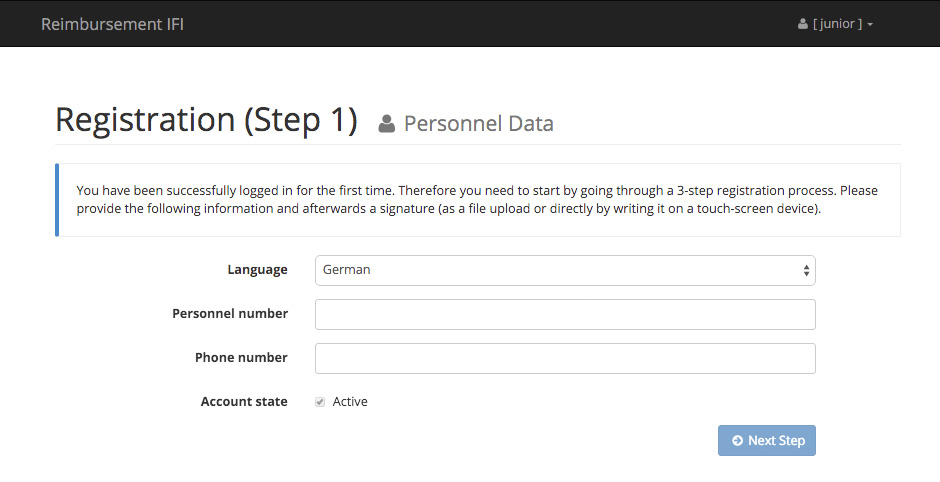
\includegraphics[width=0.80\textwidth]{registration-step01}}
    \caption{Registration step one: Capture personnel data}
    \label{fig:registration-step01}
\end{figure}

On Figure \ref{fig:registration-step02} the user has to add his signature either by uploading an image or capturing using a third party touchscreen device like a smart phone or try it in the browser. This signature is mandatory for the signature of the generated Pdf document containing all expense items.  

\begin{figure}[H]
    \centering
    \fbox{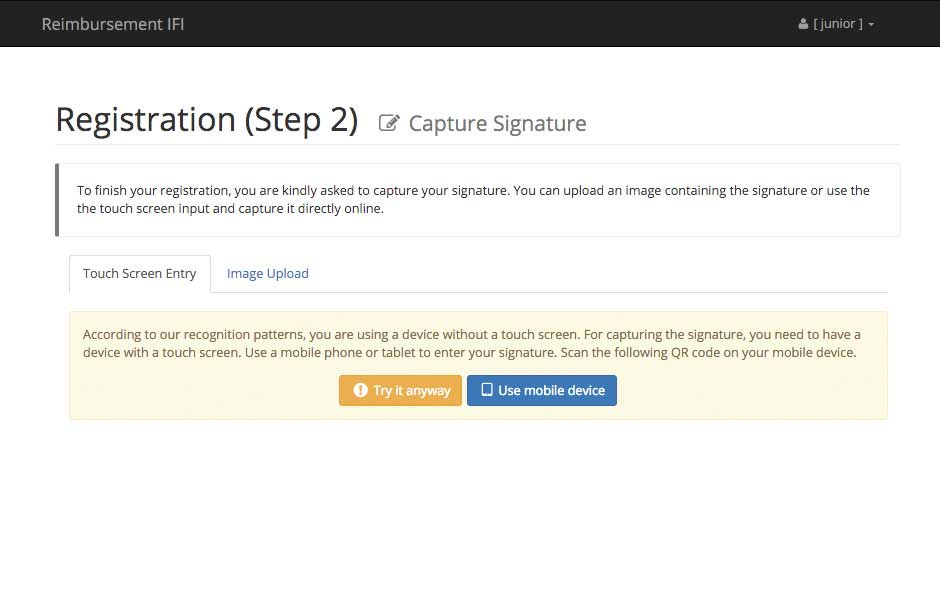
\includegraphics[width=0.80\textwidth]{registration-step02}}
    \caption{Registration step two: Capture signature}
    \label{fig:registration-step02}
\end{figure}

After completing the registration process, these captured information and signature can always be edited by going to the settings screen via the menu bar.

\section{Expenses}



\section{User}

Like user settings and roles available.



